\subsection{棱柱}\label{subsec:2-1}

\subsubsection{棱柱的概念和性质}

我们常见的一些物体,例如三棱镜、方砖以及螺杆的头部,它们都呈棱柱的形状(图 \ref{fig:ltjh-2-1})。

\begin{figure}[htbp]
    \centering
    \begin{minipage}[b]{9cm}
        \centering
        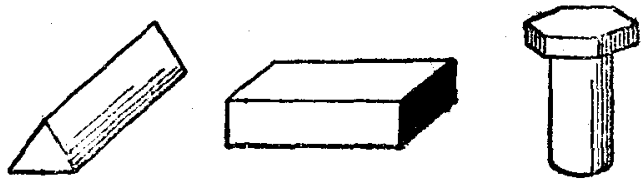
\includegraphics[width=8cm]{../pic/ltjh-ch2-01.png}
        \caption{}\label{fig:ltjh-2-1}
    \end{minipage}
    \qquad
    \begin{minipage}[b]{5cm}
        \centering
        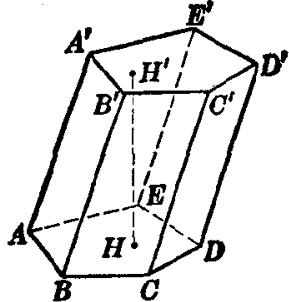
\includegraphics[width=3cm]{../pic/ltjh-ch2-02.png}
        \caption{}\label{fig:ltjh-2-2}
    \end{minipage}
\end{figure}

有两个面互相平行,其余各面都是四边形\footnote{本章所说的多边形,一般包括它内部的平面部分。},
并且每相邻两个四边形的公共边都互相平行,由这些面所围成的几何体叫做\zhongdian{棱柱}(图 \ref{fig:ltjh-2-2}),
两个互相平行的面叫做\zhongdian{棱柱的底面},其余各面叫做\zhongdian{棱柱的侧面},
两个侧面的公共边叫做\zhongdian{棱柱的侧棱},侧面与底面的公共顶点叫做\zhongdian{棱柱的顶点},
不在同一个面上的两个顶点的连线叫做\zhongdian{棱柱的对角线},两个底面间的距离叫做\zhongdian{棱柱的高}。
如图 \ref{fig:ltjh-2-2} 中的棱柱,多边形 $ABCDE$ 和 $A'B'C'D'E'$ 是底面,四边形 $ABB'A'$、$BCC'B'$ 等是侧面,
$A'A$、$B'B$ 等是侧棱,$H'H$ 是高。

棱柱用表示底面各顶点的字母来表示,如图 \ref{fig:ltjh-2-2} 中的棱柱,记作棱柱 $ABCDE{-}A'B'C'D'E'$,
或者用表示一条对角线端点的两个字母来表示,例如,棱柱 $AC'$。

\begin{figure}[htbp]
    \centering
    \begin{minipage}[b]{9cm}
        \centering
        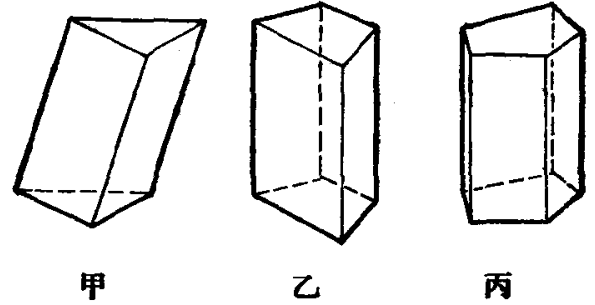
\includegraphics[width=8cm]{../pic/ltjh-ch2-03.png}
        \caption{}\label{fig:ltjh-2-3}
    \end{minipage}
    \qquad
    \begin{minipage}[b]{5cm}
        \centering
        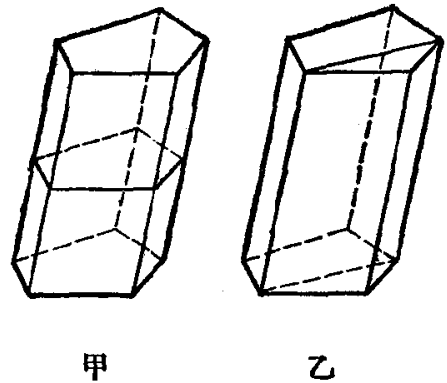
\includegraphics[width=5cm]{../pic/ltjh-ch2-04.png}
        \caption{}\label{fig:ltjh-2-4}
    \end{minipage}
\end{figure}

侧棱不垂直于底面的棱柱叫做\zhongdian{斜棱柱}(图 \ref{fig:ltjh-2-3} 甲);
侧棱垂直于底面的棱柱叫做\zhongdian{直棱柱}(图 \ref{fig:ltjh-2-3} 乙)。
底面是正多边形的直棱柱叫做\zhongdian{正棱柱}(图 \ref{fig:ltjh-2-3} 丙)。

棱柱的底面可以是三角形、四边形、五边形、…,
我们把这样的棱柱分别叫做\zhongdian{三棱柱}(图 \ref{fig:ltjh-2-3} 甲)、
\zhongdian{四棱柱}(图 \ref{fig:ltjh-2-3} 乙)、\zhongdian{五棱柱}( \ref{fig:ltjh-2-3} 丙)、 …。

根据棱柱的定义,容易得到棱柱的一些性质:

\zhongdian{(1)侧棱都相等,侧面是平行四边形;}

\zhongdian{(2)两个底面与平行于底面的截面是全等的多边形}(图 \ref{fig:ltjh-2-4} 甲);

\zhongdian{(3)过不相邻的两条侧棱的截面是平行四边形}(图 \ref{fig:ltjh-2-4} 乙)。


\begin{lianxi}

\xiaoti{求证:\zhongdian{直棱柱的侧棱长与高相等,侧面及经过不相邻的两条侧棱的截面都是矩形。}}

\xiaoti{有一个侧面是矩形的棱柱是不是直棱柱?有两个相邻侧面是矩形的棱柱呢?为什么?}

\xiaoti{斜棱柱、直棱柱和正棱柱的底面、侧面各有什么特点?}

\end{lianxi}



\subsubsection{长方体}

现在研究四棱柱的特殊情形。

底面是平行四边形的四棱柱叫做\zhongdian{平行六面体}(图 \ref{fig:ltjh-2-5} 甲)。
侧棱与底面垂直的平行六面体叫做\zhongdian{直平行六面体}(图 \ref{fig:ltjh-2-5} 乙)。
底面是矩形的直平行六面体叫做\zhongdian{长方体}(图 \ref{fig:ltjh-2-5} 丙)。
棱长都相等的长方体叫做\zhongdian{正方体}(图 \ref{fig:ltjh-2-5} 丁)。

\begin{figure}[htbp]
    \centering
    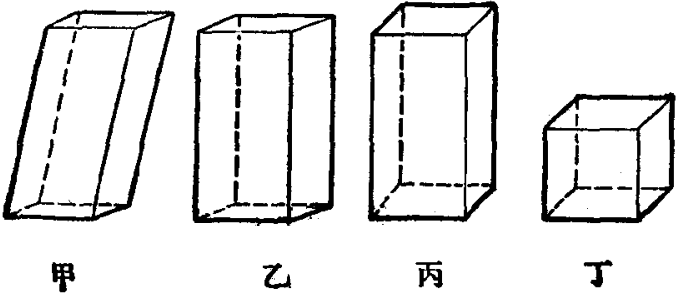
\includegraphics[width=10cm]{../pic/ltjh-ch2-05.png}
    \caption{}\label{fig:ltjh-2-5}
\end{figure}

长方体的对角线有下面的性质:

\begin{dingli}[定理][dl:cftdjx]
    长方体一条对角线长的平方等于一个顶点上三条棱的长的平方和。
\end{dingli}


已知:长方体 $AC'$ 中, $B'D$ 是一条对角线(图 \ref{fig:ltjh-2-6})。

求证:$B'D^2 = AB^2 + BC^2 + BB'\,^2$。

\zhengming 连结 $BD$,

$\because$ \quad $B'B \perp BD$,

$\therefore$ \quad $B'D^2 = BD^2 + BB'\,^2$。

又 $\because$ \quad $BD^2 = AB^2 + AD^2 = AB^2 + BC^2$,

$\therefore$ \quad $B'D^2 = AB^2 + BC^2 + BB'\,^2$。

\begin{figure}[htbp]
    \centering
    \begin{minipage}[b]{7cm}
        \centering
        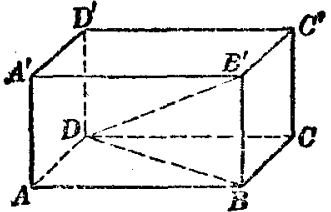
\includegraphics[width=5.5cm]{../pic/ltjh-ch2-06.png}
        \caption{}\label{fig:ltjh-2-6}
    \end{minipage}
    \qquad
    \begin{minipage}[b]{7cm}
        \centering
        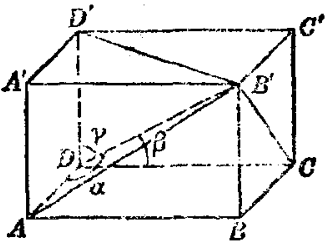
\includegraphics[width=5cm]{../pic/ltjh-ch2-07.png}
        \caption{}\label{fig:ltjh-2-7}
    \end{minipage}
\end{figure}

\liti 长方体的一条对角线与一个顶点上的三条棱所成的角分别是 $\alpha$、$\beta$、$\gamma$。 求证:
$$ \cos^2\alpha + \cos^2\beta + \cos^2\gamma = 1 \juhao $$

\begin{enhancedline}
\zhengming 连结 $AB'$、$CB'$、$D'B'$,则 $\triangle B'DA$、$\triangle B'DC$、
$\triangle B'DD'$ 都是直角三角形(图 \ref{fig:ltjh-2-7})。因此
$$ \cos\alpha = \dfrac{DA}{DB'} \douhao  \cos\beta = \dfrac{DC}{DB'} \douhao  \cos\gamma = \dfrac{DD'}{DB'} \juhao $$
将上面三个等式的两边平方后相加,得
$$ \cos^2\alpha + \cos^2\beta + \cos^2\gamma = \dfrac{DA^2 + DC^2 + DD'\,^2}{DB'\,^2} \juhao $$

又 $\because$ \quad $DB'\,^2 = DA^2 + DC^2 + DD'\,^2$,

$\therefore$ \quad $\cos^2\alpha + \cos^2\beta + \cos^2\gamma = 1$。
\end{enhancedline}

\begin{lianxi}

\xiaoti{平行六面体的各个面是什么样的四边形?直平行六面体、长方体、正方体呢?}

\xiaoti{}%
\begin{xiaoxiaotis}%
    \xxt[\xxtsep]{长方体是直四棱柱,直四棱柱是不是长方体?}

    \xxt{正方体是正四棱柱,正四棱柱是不是正方体?}

\end{xiaoxiaotis}

\xiaoti{四棱柱集合、平行六面体集合、直平行六面体集合、长方体集合、正方体集合之间有怎样的包含关系?用图表示出来。}

\end{lianxi}


\subsubsection{直棱柱直观图的画法}

前面已经研究过水平放置的平面图形的直观图的画法。
几何体的直观图的画法规则,与平面图形的画法相比,只是多画一个与 $x$ 轴、$y$ 轴都垂直的 $z$ 轴,
并且\zhongdian{平行于 $z$ 轴的线段的平行性和长度都不变。}
在直观图上,平面 $x'O'y'$ 表示水平平面,平面 $y'O'z'$ 和 $z'O'x'$ 表示直立平面。

我们以正六棱柱为例,说明直棱柱的直观图的画法。

\begin{figure}[htbp]
    \centering
    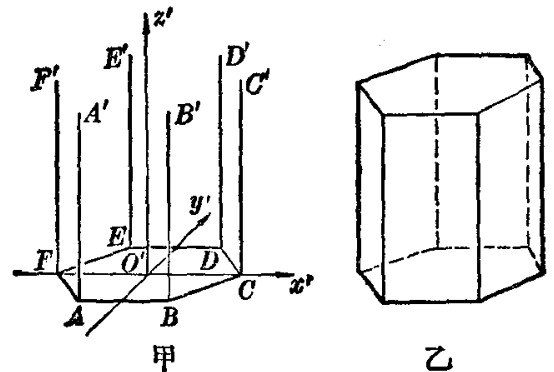
\includegraphics[width=10cm]{../pic/ltjh-ch2-08.png}
    \caption{}\label{fig:ltjh-2-8}
\end{figure}

\huafa (1)画轴 \quad 画 $x'$ 轴、$y'$ 轴、$z'$ 轴,使 $\angle x'O'y'=45^\circ$
(或 $135^\circ$), $\angle x'O'z' = 90^\circ$ (图 \ref{fig:ltjh-2-8} 甲)。

(2)画底面 \quad 按 $x'$ 轴、$y'$ 轴,画正六边形的直观图 $ABCDEF$。

(3)画侧棱 \quad 过 $A$、$B$、$C$、$D$、$E$、$F$ 各点分别作 $z'$ 轴的平行线,
并在这些平行线上分别截取 $AA'$、$BB'$、$CC'$、$DD'$、$EE'$、$FF'$ 都等于侧棱长。

(4)成图 \quad 顺次连结 $A'$、$B'$、$C'$、$D'$、$E'$、$F'$,并加以整理(去掉辅助线,
将被遮挡的部分改为虚线)。就得到正六棱柱的直观图(图 \ref{fig:ltjh-2-8} 乙)。


\subsubsection{直棱柱的侧面积}

把棱柱的侧面沿一条侧棱剪开后展在一个平面上,展开图的面积就是棱柱的侧面积。

直棱柱的侧面展开图是矩形(图 \ref{fig:ltjh-2-9}),这个矩形的长等于直棱柱底面周长 $c$,
宽等于直棱柱的高 $h$,由此我们得到下面的定理:

\begin{dingli}[定理]
    如果直棱柱的底面周长是 $c$,高是 $h$,那么它的侧面积是

    \begin{center}
       \framebox[10em]{$\bm{S_\text{直棱柱侧} = ch}$。}
    \end{center}
\end{dingli}

棱柱的全面积等于侧面积与两底面面积的和。

\begin{figure}[htbp]
    \centering
    \begin{minipage}[b]{7cm}
        \centering
        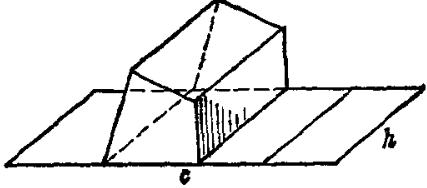
\includegraphics[width=7cm]{../pic/ltjh-ch2-09.png}
        \caption{}\label{fig:ltjh-2-9}
    \end{minipage}
    \qquad
    \begin{minipage}[b]{7cm}
        \centering
        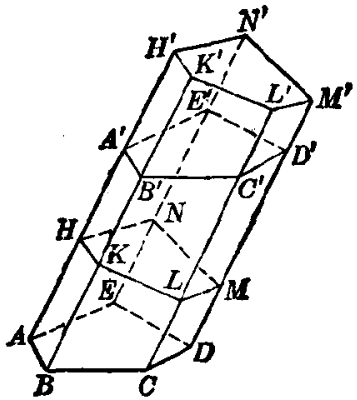
\includegraphics[width=4.5cm]{../pic/ltjh-ch2-10.png}
        \caption{}\label{fig:ltjh-2-10}
    \end{minipage}
\end{figure}

\liti 求证:斜棱柱的侧面积等于它的直截面(垂直于侧棱的截面)的周长与侧棱长的乘积。

已知:如图 \ref{fig:ltjh-2-10},斜棱柱 $AC'$ 的侧棱长是 $l$,直截面 $HKLMN$ 的周长是 $c_1$。

求证: $S_\text{斜棱柱侧} = c_1l$。

证明:延长侧棱 $AA'$ 到 $H'$, 使 $A'H' = AH$。
设过 $H'$ 平行于直截面 $HKLMN$ 的平面,与各侧棱的延长线交于 $K'$、$L'$、$M'$、$N'$。
这样,就得到一个以斜棱柱的直截面为底,侧棱长为高的直棱柱 $HL'$(图 \ref{fig:ltjh-2-10})。

因为 $\text{底面}\;H'L' \pingxing \text{底面}\;HL$,
它们的公垂线段 $HH' = KK' =LL' = \cdots = NN' = AA' = l$,所以,
斜棱柱 $AC'$ 的各侧面的面积与直棱柱 $HL'$ 中对应的侧面面积相等。 因此
$$ S_\text{斜棱柱侧} = S_\text{直棱柱侧} = c_1 \cdot HH' \juhao $$

即 \quad $S_\text{斜棱柱侧} = c_1l$。

实际上,在本题的证明中,是把斜棱柱 $AC'$ 的直截面下面的一部分,移动一下位置,与另一部分组成直棱柱 $HL'$。


\begin{lianxi}

\xiaoti{画一个底面边长是 3 cm,高是 4.5 cm 的正三棱柱的直观图(不写画法)。}

\xiaoti{已知正六棱柱的高为 $h$,底面边长为 $a$,求全面积。}

\end{lianxi}

